En esta sección se presentan los resultados empíricos obtenidos. Los gráficos se han generado de forma automatizada a partir de los datos recolectados, permitiendo contrastar el rendimiento práctico de los algoritmos con su complejidad teórica en el modelo word-RAM.

\subsection{Ordenamiento de Arreglos}

Se evaluó el comportamiento de los cuatro algoritmos (\textit{Standard Sort}, \textit{Merge Sort}, \textit{Quick Sort} y \textit{Patience Sort}) bajo distintos tamaños de entrada ($n$) midiendo tanto el tiempo de ejecución como el consumo de memoria.

\subsubsection{Análisis de Tiempo de Ejecución}

\begin{figure}[H]
    \centering
    \begin{minipage}{0.48\textwidth}
        \centering
        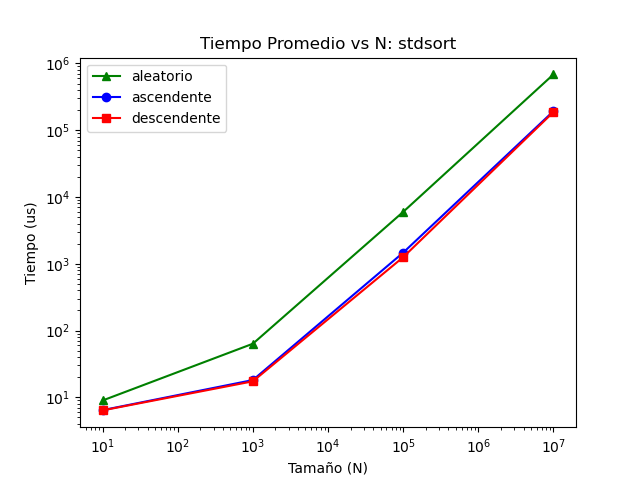
\includegraphics[width=0.85\linewidth]{code/sorting/data/plots/tiempo_stdsort.png}
        \caption{Tiempo: Std Sort}
        \label{fig:time_std}
    \end{minipage}\hfill
    \begin{minipage}{0.48\textwidth}
        \centering
        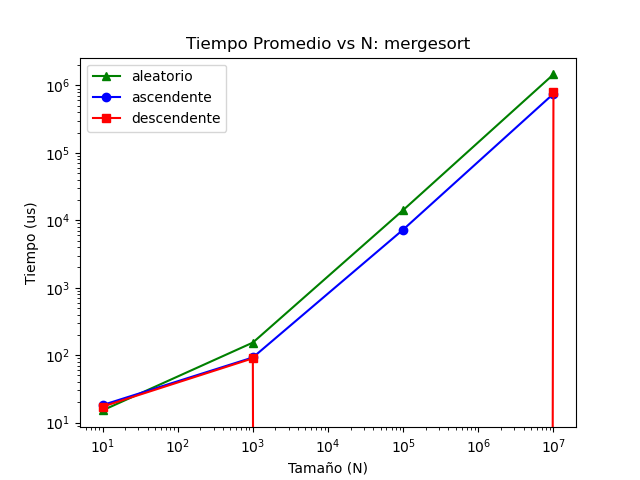
\includegraphics[width=0.85\linewidth]{code/sorting/data/plots/tiempo_mergesort.png}
        \caption{Tiempo: Merge Sort}
        \label{fig:time_merge}
    \end{minipage}

    \vspace{0.4cm}

    \begin{minipage}{0.48\textwidth}
        \centering
        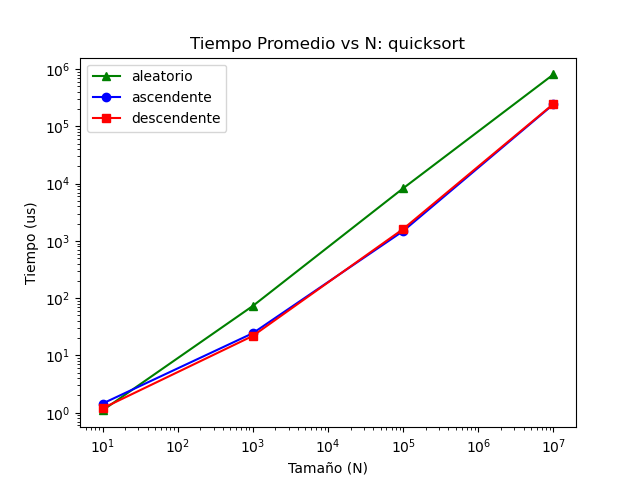
\includegraphics[width=0.85\linewidth]{code/sorting/data/plots/tiempo_quicksort.png}
        \caption{Tiempo: Quick Sort}
        \label{fig:time_quick}
    \end{minipage}\hfill
    \begin{minipage}{0.48\textwidth}
        \centering
        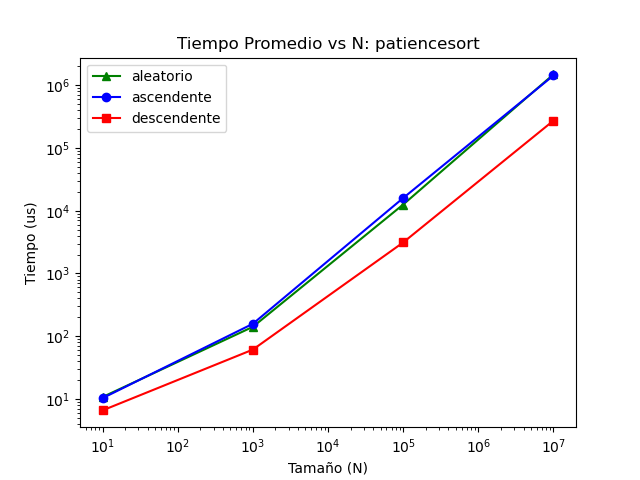
\includegraphics[width=0.85\linewidth]{code/sorting/data/plots/tiempo_patiencesort.png}
        \caption{Tiempo: Patience Sort}
        \label{fig:time_patience}
    \end{minipage}
\end{figure}

Al observar el tiempo de ejecución, \textit{Standard Sort} y \textit{Quick Sort} (Figuras \ref{fig:time_std} y \ref{fig:time_quick}) muestran rendimientos muy eficientes. Esto se alinea con la teoría que establece que, en arreglos con orden aleatorio, el árbol de recursión de Quick Sort es balanceado en promedio, logrando un costo asintótico proporcional a $n \log n$. Por otro lado, \textit{Merge Sort} (Figura \ref{fig:time_merge}) presenta tiempos estables pero es un poco más lento; esto ocurre porque ejecuta exactamente $2n$ asignaciones de elementos en arreglos auxiliares durante la fase de mezcla. 

Un caso de estudio fundamental es \textit{Patience Sort} (Figura \ref{fig:time_patience}), el cual exhibe una dependencia crítica de la distribución inicial. En arreglos ascendentes, el algoritmo es forzado a crear $N$ pilas distintas, maximizando el trabajo del \textit{min-heap} y disparando el tiempo de ejecución. En contraste, ante un arreglo descendente, todos los elementos se apilan sobre una única estructura, eludiendo el peor caso y resolviendo el problema con una eficiencia casi lineal.

Cabe notar que la línea de \textit{Merge Sort} descendente (Figura \ref{fig:time_merge}) presenta saltos abruptos en $n = 10^3$ y $n = 10^5$. Al inspeccionar el archivo de mediciones, se identificó que 2 de las 1756 muestras registradas
(0,11\,\%) presentaron duraciones negativas imposibles (del orden de $-10^6\,\mu s$), lo que distorsiona el promedio de esos puntos en la escala logarítmica del gráfico. Este artefacto es atribuible a una desincronización puntual del reloj bajo el entorno WSL2 durante esas corridas específicas, y no refleja el comportamiento real del algoritmo: al excluir esas dos muestras, la curva resultante es consistente con la tendencia $n \log n$ esperada y con el comportamiento observado en \textit{Std Sort} y \textit{Quick Sort} (Figura \ref{fig:time_std} y \ref{fig:time_quick}). El fenómeno no afecta ninguna de las conclusiones del informe.

\subsubsection{Análisis de Consumo de Memoria}

\begin{figure}[H]
    \centering
    \begin{minipage}{0.48\textwidth}
        \centering
        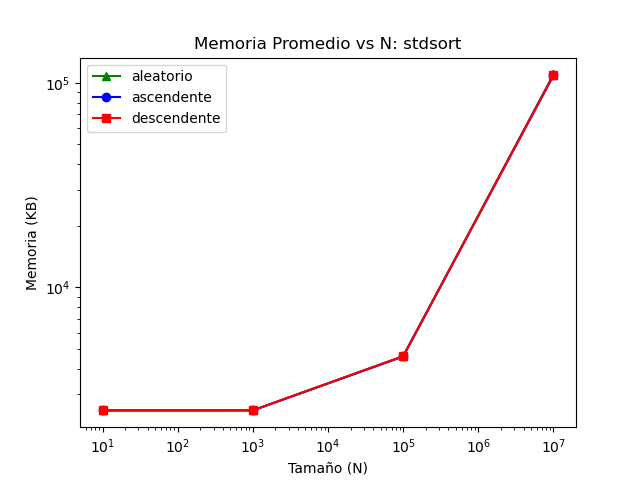
\includegraphics[width=0.85\linewidth]{code/sorting/data/plots/memoria_stdsort.png}
        \caption{RAM: Std Sort}
        \label{fig:mem_std}
    \end{minipage}\hfill
    \begin{minipage}{0.48\textwidth}
        \centering
        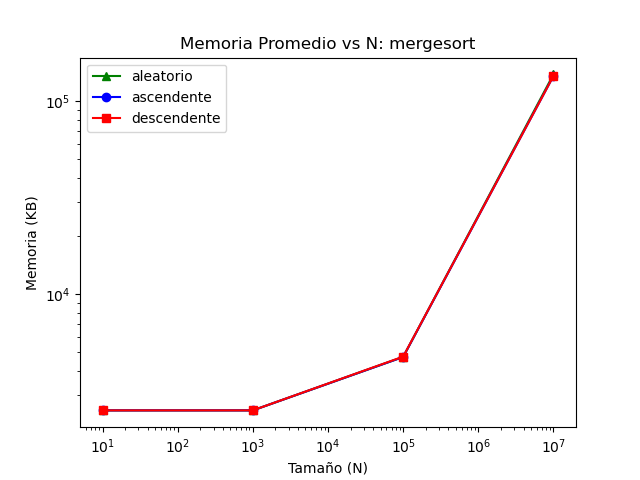
\includegraphics[width=0.85\linewidth]{code/sorting/data/plots/memoria_mergesort.png}
        \caption{RAM: Merge Sort}
        \label{fig:mem_merge}
    \end{minipage}

    \vspace{0.4cm}

    \begin{minipage}{0.48\textwidth}
        \centering
        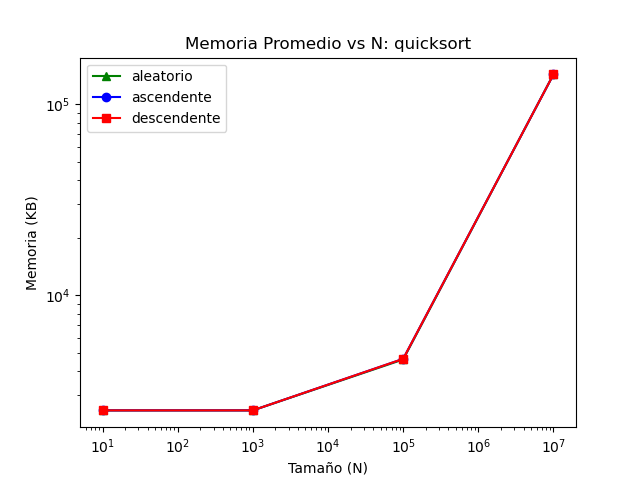
\includegraphics[width=0.85\linewidth]{code/sorting/data/plots/memoria_quicksort.png}
        \caption{RAM: Quick Sort}
        \label{fig:mem_quick}
    \end{minipage}\hfill
    \begin{minipage}{0.48\textwidth}
        \centering
        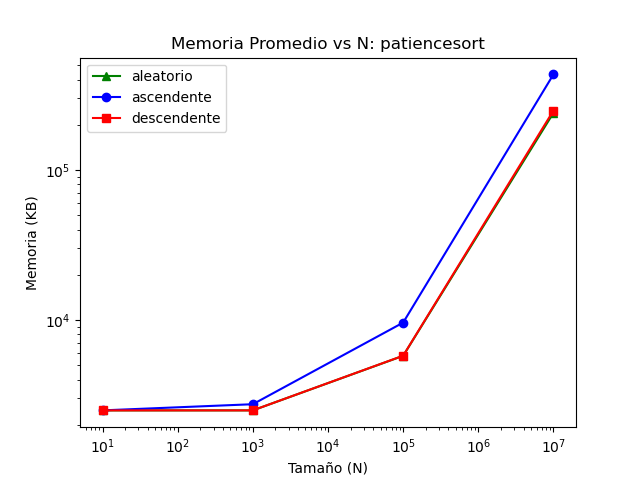
\includegraphics[width=0.85\linewidth]{code/sorting/data/plots/memoria_patiencesort.png}
        \caption{RAM: Patience Sort}
        \label{fig:mem_patience}
    \end{minipage}
\end{figure}

El uso real de memoria refleja las características estructurales de cada algoritmo. \textit{Quick Sort} (Figura \ref{fig:mem_quick}) logra mantener un perfil bajo de memoria ya que particiona el arreglo de forma \textit{in-place}. Sin embargo, debido al espacio requerido por la pila de llamadas recursivas \textit{(call-stack)}, utiliza una cantidad $O(\log n)$ de memoria adicional en el caso promedio \cite{gfg_quicksort}. Por otro lado, la Figura \ref{fig:mem_merge} evidencia que \textit{Merge Sort} exige un arreglo temporal adicional, implicando un uso de espacio $\Theta(n)$ para realizar la mezcla de las mitades \cite{taocv3, gfg_mergesort_algo}. Este fenómeno estructural también castiga a \textit{Patience Sort} en su peor caso (Figura \ref{fig:mem_patience}), donde la creación de $N$ pilas individuales en arreglos ascendentes dispara el consumo de RAM, separándose drásticamente de su rendimiento en arreglos descendentes.

\subsection{Multiplicación de Matrices}

Finalmente, se exponen los resultados para los enfoques \textit{Naive} y \textit{Strassen}, midiendo tanto tiempo de ejecución como consumo de RAM para matrices cuadradas.

\begin{figure}[H]
    \centering
    \begin{minipage}{0.48\textwidth}
        \centering
        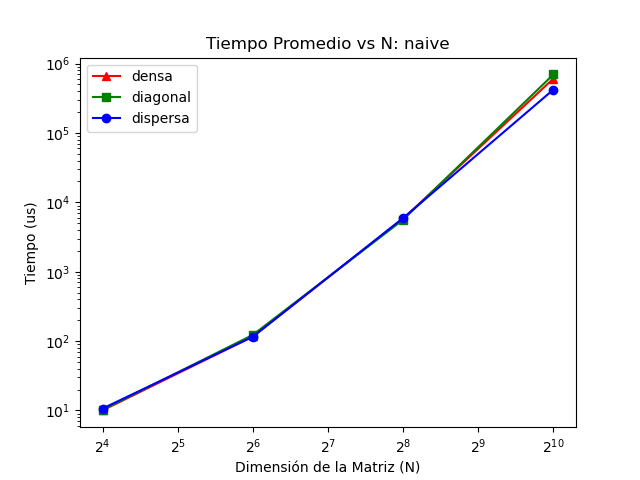
\includegraphics[width=0.85\linewidth]{code/matrix_multiplication/data/plots/tiempo_naive.png}
        \caption{Tiempo: Naive.}
        \label{fig:mat_time_naive}
    \end{minipage}\hfill
    \begin{minipage}{0.48\textwidth}
        \centering
        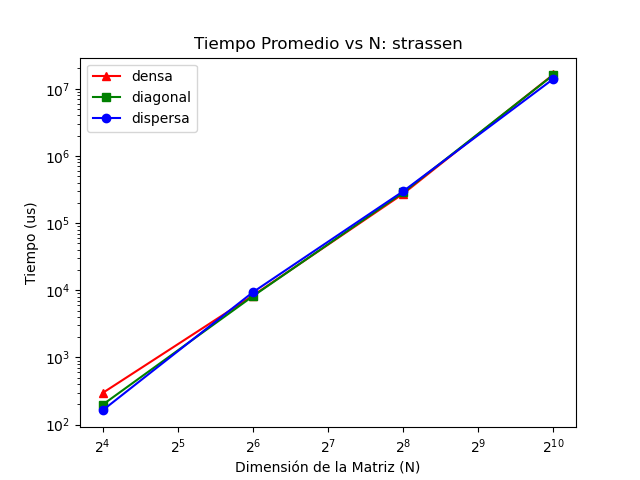
\includegraphics[width=0.85\linewidth]{code/matrix_multiplication/data/plots/tiempo_strassen.png}
        \caption{Tiempo: Strassen.}
        \label{fig:mat_time_strassen}
    \end{minipage}
    
    \vspace{0.4cm}
    
    \begin{minipage}{0.48\textwidth}
        \centering
        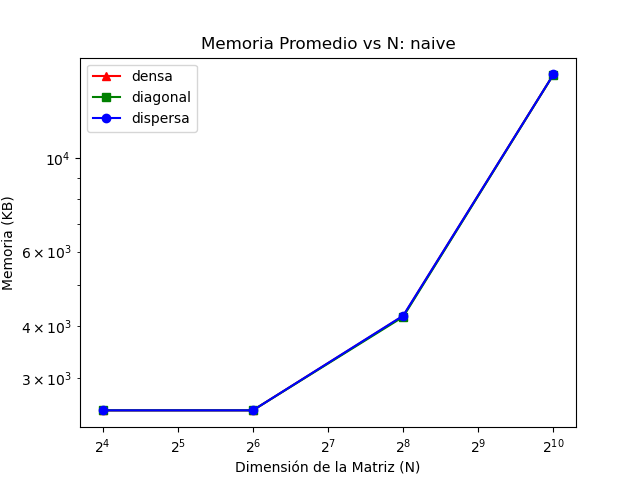
\includegraphics[width=0.85\linewidth]{code/matrix_multiplication/data/plots/memoria_naive.png}
        \caption{RAM: Naive.}
        \label{fig:mat_mem_naive}
    \end{minipage}\hfill
    \begin{minipage}{0.48\textwidth}
        \centering
        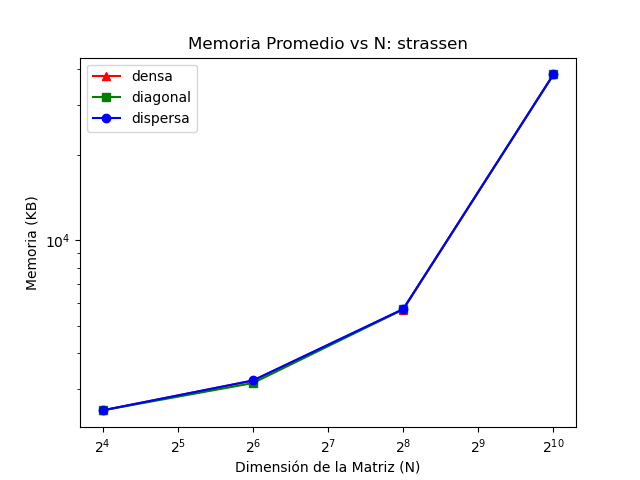
\includegraphics[width=0.85\linewidth]{code/matrix_multiplication/data/plots/memoria_strassen.png}
        \caption{RAM: Strassen.}
        \label{fig:mat_mem_strassen}
    \end{minipage}
\end{figure}

Aunque teóricamente la cota de Strassen, definida por $\Theta(n^{\log_2 7})$, crece más lento y debería dominar en eficiencia temporal a la cota ajustada $\Theta(n^3)$ del algoritmo Naive para valores grandes de $n$ \cite{algorithms_erickson}, empíricamente se observa que \textit{Naive} es consistentemente más rápido para todas las dimensiones evaluadas (hasta $n=2^{10}$). Esta victoria empírica no solo ocurre por las altas constantes ocultas y la excesiva sobrecarga de memoria dinámica que exige el diseño recursivo de Strassen \cite{castillo_apuntes}. El factor decisivo es la localidad de referencia: la implementación de \textit{Naive} altera el orden de los bucles a $i-k-j$, logrando acceder a la memoria de la segunda matriz de forma contigua. Esto evade casi por completo los fallos de caché (\textit{cache misses}), acelerando la ejecución de una forma que el análisis asintótico tradicional no logra capturar.
